
%(BEGIN_QUESTION)
% Copyright 2011, Tony R. Kuphaldt, released under the Creative Commons Attribution License (v 1.0)
% This means you may do almost anything with this work of mine, so long as you give me proper credit

An electronic temperature transmitter has an input range of 100 to 500 degrees Fahrenheit (type J thermocouple) and an output range of 4 to 20 mA.  When subjected to a series of simulated temperatures (5-point up/down test), it responds as such:

% No blank lines allowed between lines of an \halign structure!
% I use comments (%) instead, so that TeX doesn't choke.

$$\vbox{\offinterlineskip
\halign{\strut
\vrule \quad\hfil # \ \hfil & 
\vrule \quad\hfil # \ \hfil \vrule \cr
\noalign{\hrule}
%
% First row
Simulated temperature & Output signal \cr
%
% Another row
(deg F) & (mA) \cr
%
\noalign{\hrule}
%
% Another row
100 & 4.1 \cr
%
\noalign{\hrule}
%
% Another row
200 & 8.0 \cr
%
\noalign{\hrule}
%
% Another row
300 & 11.75 \cr
%
\noalign{\hrule}
%
% Another row
400 & 16.0 \cr
%
\noalign{\hrule}
%
% Another row
500 & 20.2 \cr
%
\noalign{\hrule}
%
% Another row
400 & 16.0 \cr
%
\noalign{\hrule}
%
% Another row
300 & 11.75 \cr
%
\noalign{\hrule}
%
% Another row
200 & 8.0 \cr
%
\noalign{\hrule}
%
% Another row
100 & 4.1 \cr
%
\noalign{\hrule}
} % End of \halign 
}$$ % End of \vbox

Graph this instrument's ideal transfer function on the graph below, along with its {\it actual} transfer function graph based on the measured values recorded above.  Then, determine what kind of calibration error it has ({\it zero shift}, {\it span shift}, {\it linearity}, and/or {\it hysteresis}).

$$\includegraphics[width=15.5cm]{i03489x01.eps}$$

\vfil 

Hint: a computer spreadsheet program might be a useful tool in graphing this instrument's response.  Feel free to attach a printed copy of a spreadsheet graph instead of hand-sketching one on this page.

\underbar{file i03489}
\eject
%(END_QUESTION)





%(BEGIN_ANSWER)

This is a graded question -- no answers or hints given!

%(END_ANSWER)





%(BEGIN_NOTES)

This transmitter definitely has a {\it linearity} error, and one could say it has {\it zero} and {\it span} errors as well:

$$\includegraphics[width=15.5cm]{i03489x02.eps}$$

%INDEX% Calibration errors, identifying

%(END_NOTES)

